Every time a scientist creates or implements a model, it is important to verify that the model is giving correct results. Or maybe we should rephrase; it is important to verify that the model is \textit{doing as intended}. It is not always clear what correct results \textit{means}. As George E.P. Box said
\begin{aquote}{George E.P. Box, 1987}
Essentially, all models are wrong, but some are useful.
\end{aquote}
A good model should be in agreement with already existing theories (at least those we believe are reliable). Take special relativity for example, in the limit of low velocities, it reproduces the results of Newtonian mechanics (e.g. the effects time dilation and length contraction vanishes). In this chapter we will first validate the model by comparing the outcome of the model to established theoretical results in section \ref{sec:dsmc_code_validation}. In section \ref{sec:dsmc_parallelization_performance} we discuss how well the performance of the implementation scales for an increasing number of processors. We then, in section \ref{sec:results_for_simple_geometries}, analyze the Knudsen correction for the permeability for flow in a cylinder for various Knudsen numbers and cylinder radii. We conclude the chapter by studying a more complicated geometry, randomly packed spheres, in section \ref{sec:dsmc_packed_spheres_results}.

\section{Code validation}
\label{sec:dsmc_code_validation}
We validate the DSMC implementation by comparing numerical results to those of statistical mechanics and the kinetic theory. First we let the particles start in some non-equilibrium state where all the velocity components are $\pm v_0$ to confirm that the collision model results in the Maxwell-Boltzmann velocity distribution. The velocity $v_0$ corresponds to some initial temperature $T_0$ that defines the standard deviation in the Maxwell-Boltzmann distribution. Then we study the Poisuille flow (two infinite parallel plates) and compare the spatial velocity distribution $v(x)$ - $x$ being the distance from the lower plate - to numerical solutions to the linearized Boltzmann equation.
\subsection{Maxwell-Boltzmann velocity distribution}
We showed in section \ref{sec:maxwell_boltzmann_distribution} that the particles in a gas in equilibrium will have velocities according to the Maxwell-Boltzmann distribution. We have run a simulation with $10^5$ simulated particles with initial velocities given for each particle $n$ as
\begin{align}
	\nonumber
	\dot x_n &= v_0(1 - 2 (n\bmod 2))\\
	\label{eq:weird_velocity_distribution}
	\dot y_n &= v_0(1 - 2 ((n+1)\bmod 2))\\
	\nonumber
	\dot z_n &= \dot x_n,
\end{align}
where $v_0$ is some velocity chosen so that $T\approx 300K$. There are no walls the particles can exchange energy with, so the total energy is conserved. The reason we have chosen this initial velocity distribution is that the net momentum will be zero if $N$ is an even number (each particle's velocity components is canceled out by the next particle). This is is of course not the Maxwell-Boltzmann distribution - we are not in an equilibrium state. We expect that after some time, the system will equilibrate and approach the Maxwell-Boltzmann distribution which is given as (equation \eqref{eq:maxwell_boltzmann_distribution})
\begin{align}
	P(v_i)\dm {v_i} = \sqrt{m\over 2\pi k_BT}e^{-mv_i^2\over 2k_BT}\dm {v_i},
\end{align}
where $i\in \{x,y,z\}$ indicates the velocity component. We ran the simulation for $10^5$ timesteps, and as we see in figure \ref{fig:velocity_distribution}, the collision algorithm reproduces this distribution perfectly. The temperature that was measured to be $T=\unit{298.5}{\kelvin}$.
\begin{figure}[htb]
\begin{center}
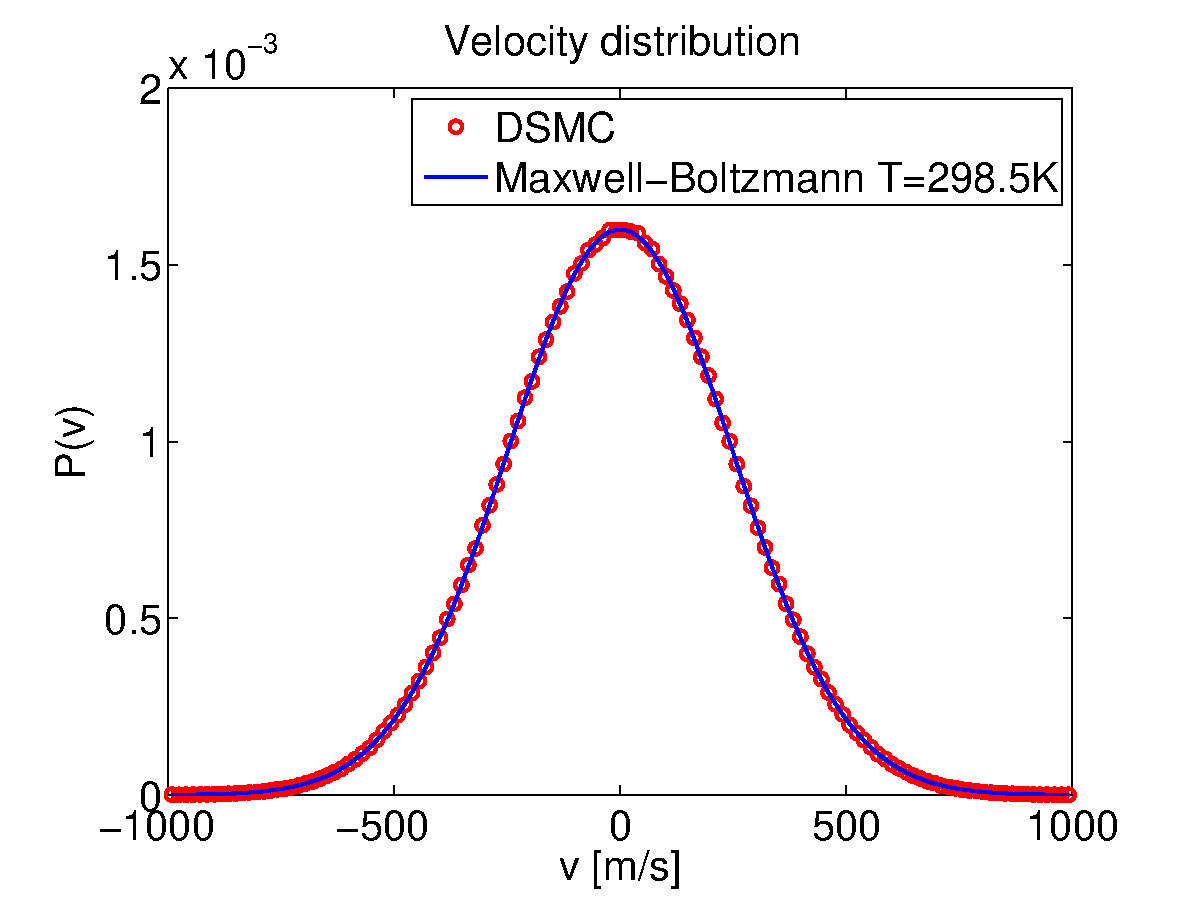
\includegraphics[width=0.7\textwidth, trim=0cm 0cm 0cm 0cm, clip]{DSMC/figures/velocity_distribution.eps}
\end{center}
\caption{The system clearly reaches the Maxwell-Boltzmann distribution when the initial velocity distribution follows equation \ref{eq:weird_velocity_distribution}. Here the final temperature was measured to $T=$\unit{298.5}{\kelvin} which reproduces the expected distribution perfectly.}
\label{fig:velocity_distribution}
\end{figure}

\subsection{Poiseuille velocity profile}
\label{sec:dsmc_validation_poiseuille}
The Poiseuille flow through a long channel is a standard and fundamental problem that is widely studied in the gas dynamics literature. The system consists of two infinite parallel plates, displaced by a distance $h$ in the $y$-direction. A pressure gradient is applied in the $z$-direction by a constant acceleration $g$ corresponding to equation \ref{eq:acceleration_to_pressure_difference}. The channel is periodic in the $x$ and $z-$direction, emulating a large system with negligible boundary effects. The gas particles collide with the plates through the thermal wall model, so the reflected particles will have zero tangential velocity on average. In the continuum limit, $\text{Kn}\rightarrow 0$, we expect the velocity profile to approach the parabolic solution \cite{batchelor2000introduction}
\begin{align}
	v_z(y) = \nabla P\frac{1}{2\mu}y(y-h).
\end{align}
However, in the transition flow regime, $0.1 \leq \text{Kn} \leq 10$, we expect a non zero slip velocity\cite{morris1992slip}. The Knudsen number will affect the velocity distribution through the fact that a high Knudsen number means a larger mean free path, hence fewer inter-molecular collisions. A low collision rate will make the surface effects propagate slower through the system resulting in a higher slip velocity. Ohwada et al. \cite{ohwada1989numerical} studied the Poiseuille flow for hard-sphere molecules with a wide range of Knudsen numbers by numerically solving the linearized Boltzmann equation. By using non-dimensionalized units, the result is not dependent on the pressure difference or the temperature. The only assumption is that the pressure gradient is so small that the Boltzmann equation can be linearized around the equilibrium state. To set up as system like this is a simple task with the DSMC algorithm, and is a good test case to validate both the surface interaction model and the inter-molecular collision model.

We chose a cubic system with side length \unit{1.0}{\micro\meter} with a solid plate at $y=$\unit{0}{\micro\meter} and $y=$\unit{1.0}{\micro\meter}. We ran six simulations with different densities, corresponding to different Knudsen numbers in the range $[0.1, 11.0]$. We want to vary the Knudsen number which was defined as
\begin{align}
	\text{Kn} = \frac{\lambda}{L} = \frac{1}{\sqrt 2 \pi d^2 \rho_n L}.
\end{align}
We have substituted the mean free path from equation \eqref{eq:mean_free_path} in the last expression so that we can choose the Knudsen number through the density
\begin{align}
	\rho_n(\text{Kn}) = \frac{1}{\sqrt 2 \pi d^2 \text{Kn}L}.
\end{align}
In all runs, we chose the number of real atoms per particle $N_\text{eff}$ = 10. Assuming ideal gas pressure $P_0$, an applied pressure difference corresponding to $0.1P_0$ was chosen to induce the flow. In figure \ref{fig:dsmc_validation_poiseuille} we see that the velocity profiles produced from the DSMC model is in excellent agreement with the solutions obtained by Ohwada et al. for all Knudsen numbers. We also see that as the Knudsen number increases, the slip velocity also increases, which is what we expect, see section \ref{sec:slip_length}.
\begin{figure}[htpb]
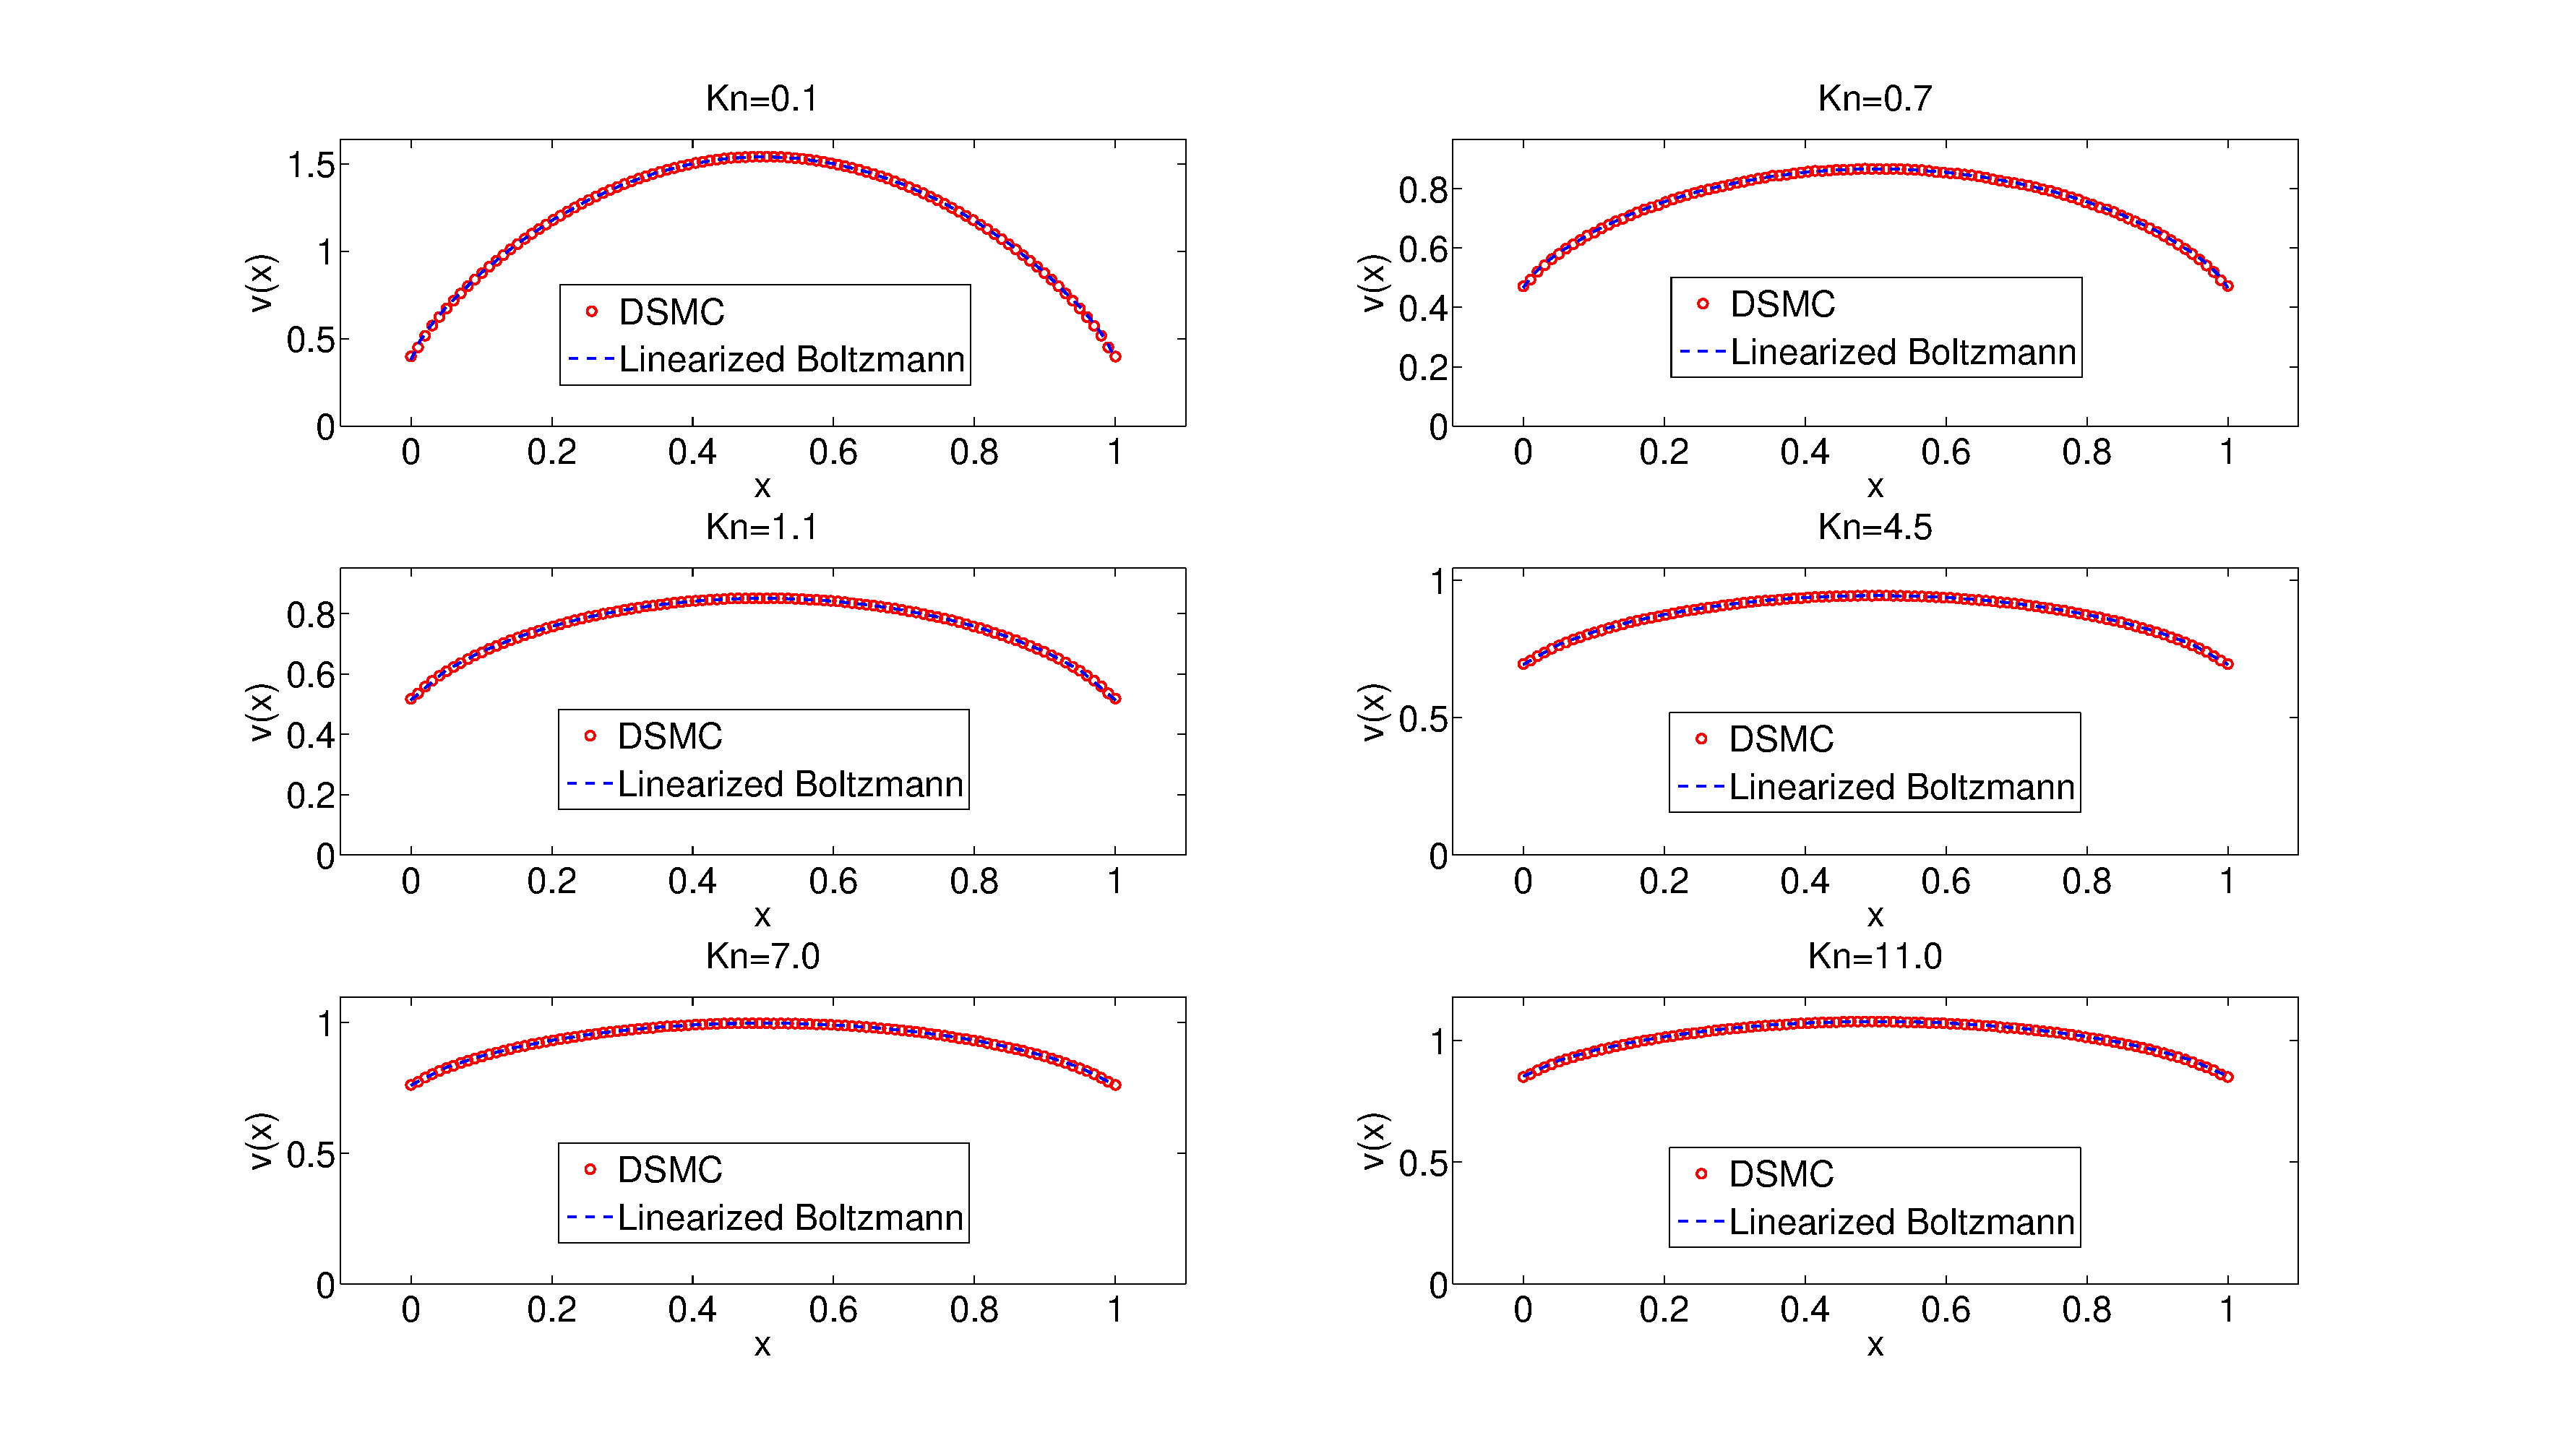
\includegraphics[width=\textwidth, trim=6cm 0cm 5cm 0cm, clip]{DSMC/figures/validation_poiseuille.eps}
\centering
\caption{Non-dimensionalized velocity distribution for flow between infinite parallel thermal plates for different Knudsen numbers over two orders of magnitude. Each run is compared to the linearized Boltzmann solution of Ohwada et al\cite{ohwada1989numerical} which shows that the algorithm produces correctly the behavior in all regions, near the wall and internally in the channel. An applied pressure difference $\Delta P = P_A - P_B$ with $P_A = 1.1P_B$ is applied. The initial temperature is $T$=\unit{300}{\kelvin}. We see how the slip velocity becomes larger for increasing Knudsen numbers, as expected from the discussion in section \ref{sec:slip_length}. }
\label{fig:dsmc_validation_poiseuille}
\end{figure}